\chapter{Proposed Approach}

% \begin{itemize} 
% 	\item describe everything you yourself did (as opposed to the fundamentals chapter, which explains what you built on)
% 	\item start with a theoretical approach    
% 	\item describe the developed system/algorithm/method from a high-level point of view
% 	\item go ahead in presenting your developments in more detail  
% 	\item recommended length: approximately one third of the thesis.
% \end{itemize}

Different approaches are presented and discussed in this chapter using data link unicast or broadcast in different specifications,
these were also empirically tested and evaluated in the \cref{sec:evaluation}.
At the end of this chapter, the test setup will be introduced and 
it is briefly explained how the chips are programmed.

\section{Design}

\begin{table}[h]
	\centering
	% \label{tab:layer_overview}
	\begin{tabular} { ccc }
		\begin{tabular}{ |c| } 
			\hline
			Art-Net\\
			\hline
			UDP\\
			\hline
			IP\\
			\hline
			802.11 DL/Unicast\\
			\hline
			802.11* PHY\\ 
			\hline
		\end{tabular}
		\begin{tabular}{ |c| } 
			\hline
			Slim Application\\
			\\
			\\
			\hline
			802.11 DL/UC or BC\\
			\hline
			802.11* PHY\\ 
			\hline
		\end{tabular}
	\end{tabular}
	\caption{Art-Net Layer compared with Slim Data Link Layer}
	\label{tab:Layer}
\end{table}

The use of high-layer protocols, such as Art-Net \cref{sec:artnet}, in lighting technology involves a considerable overhead. 
Because the lighting console does not talk directly to the \ac{WES}, communication must be controlled via an \ac{AP}, 
which means that the \ac{IP} (layer 3) must be used for addressing and \ac{UDP} (layer 4) for transporting the data. 
They both come withe additional headers. 
Such an overhead can lead to latency, channel congestion and packet loss.
 
In an ad-hoc network \cref{itm:bss}, on the other hand, packets can be sent directly on the MAC (layer 2) \cref{tab:Layer}. 
With a payload of a few bytes to each WES, keeping overheat small can be quite important. 
Complexity problems as often typical in Ad-Hoc networks are not to be assumed, 
since the controller at the light desk must normally stand in line of sight to the individual WES, 
from there finally the lighting technician from there must have everything in the range of vision to be able to intervene. 
One can therefore assume a simple star topology.
In the following the ESP-NOW \cref{sub:espnow} protocol was chosen to distribute the packets low-level, 
because even if it was not developed for this purpose the specification fits quite well to the requirements.

\todo{topology of data flow isnt linked in the text}
\begin{figure}[h]
	\centering
	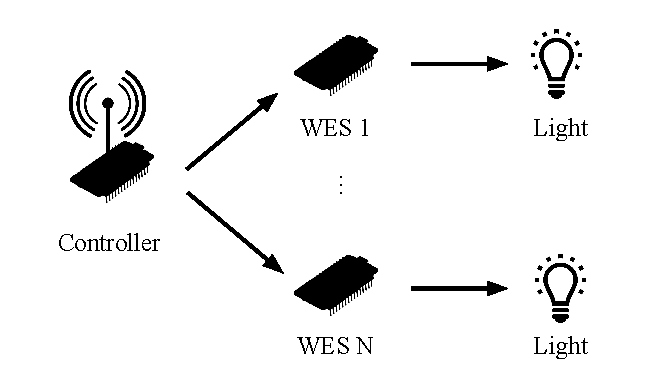
\includegraphics[scale=0.75]{figures/dataFlow.pdf}
	\caption{Topology of the Data Flow}
	\label{fig:testbed}
\end{figure}

For the purpose of this analysis, the controller transmits 20 byte (analogue to 20 DMX channels) to every WESs.
Four different metrics are considered, which where discussed in the requirements.
\begin{itemize}
	\item \textbf{Latency} \\
	What is the latency from commanding the controller to the estimated reaction at the WES e.g. lighting of a light?
	For the sake of simplicity, delays caused by the microcontroller instruction set, data distribution and 
	control of the light installation are neglected and the focus is placed only on the airtime.
	Low latency is important so that the lighting technician can intervene live in the light show,
	but the lights do not react with delay.
	\item \textbf{Update Frequency}\\
	How often can the we update all WESs per second? 
	This results in how smooth movement of moving heads are moving or how smooth the transition
	of the color of an LED can be performed
	and the control can be adapted rhythmically to the musical beat.
	\item \textbf{Reliability}\\
	Wie sicher kommen die vom Controller gesendeten Daten bei den WESs an?
	Lack of reliability can result 
	in two WESs positioned next to each other not behaving the same because one of them only receives half of the signals.
	\item \textbf{Synchronisation}\\
	Are the signals sent to different WESs carried out at the same time?
	If two of the WESs are to be controlled simultaneously, 
	but the signal was transmitted one after the other, they have to wait for each other so that the lights change at the same time.
\end{itemize}

\subsection*{Slim Unicast}

The implementation that probably comes closest to Art-Net's is to replace the TCP packets sent by Art-Net 
to the respective IP-Address of the WESs with unicasts to the MAC-address of the WES.
Of course, the MAC address of all WESs must be known and they must all be paired with the controller, but 
this process is just analogous to  mapping the corresponding IP addresses after dialing the WESs into a WLAN.

\subsubsection*{Latency}

Latency describes the time between a command and the expected response, here considered as airtime.
The airtime using 1Mbit/s is rather easy calculated, every byte (8 Bits) takes 8$\mu$s.

For a full transmission the PHY and MAC preamble and header be transmitted twice, once for the data and once for the acknowledgement.
The MAC body contains the payload, which depends of the needs of the addressed \ac{WES}.
In a perfect clean channel the sender hasn't to defer, but has to take a \ac{DIFS} plus a backoff.
A perfect empty channel resets the CW to CW$_{min}$, which are 31 slots in 802.11b
and a slot time of 20$\mu$s an average delay of $370\mu$s is estimated.

\begin{align}
	\frac{CW_{min}}{2}=\frac{31}{2}=16.5 \\
	20\mu s \cdot 16.5 = 370\mu s
\end{align}

\begin{table}[h]
	\centering
	\begin{tabular} { lrr }
		\toprule
		\multicolumn{1}{c}{Frame segment}
		& \multicolumn{1}{c}{Byte}
		& \multicolumn{1}{c}{Duration in $\mu$s} \\
		\midrule
		DIFS								& -		& 50 \\
		Average Backoff						& -		& 370 \\
		PHY header: PLCP preamble			& 18	& 144 \\
		PHY header: PLCP header				& 6 	& 48 \\
		MAC headers							& 28	& 224 \\
		MAC body							& 20 	& 160 \\
		\textbf{= tx time data}				& 		& \textbf{956} \\
		SIFS								& -		& 10 \\
		PHY header: PLCP preamble			& 18	& 144 \\
		PHY header: PLCP header				& 6		& 48 \\
		MAC headers, no MAC body	 		& 18	& 112 \\
		\textbf{= tx time ack}				& 		& \textbf{314} \\
		\bottomrule
	\end{tabular}
	\caption{Composition of the Total Airtime (tx + ack)}
	\label{tab:airtime_unicast_calc}
\end{table}

The total airtime of the transmission of data and ack, assuming the transmission arrived successfully, is $t_tx=1100\mu$s.
Strictly speaking, the light could also be changed before the acknolegement is sent, i.e. after 956$\mu$s.
The latency scales linearly, the delay to the n-th WES is:
\begin{align}
	\text{Airtime} = N \cdot t_{tx} = N \cdot 1270\mu s
\end{align}

In order to avoid unnecessary load on the radio channel, Art-Net transmit only the changes.
In the worst case, however, changes affect all WESs at the same time.

\subsubsection*{Update Frequency}
Following the approach of DMX and updating the 'bus' every 44Hz, would made by sending the packets round robin via unicast. 
With a correspondingly high number of WESs, this could be challenge with a transmission speed of 1MBit/s, 
it also scales linearly with each additional WES. 
In an labor steril empty channel, denying all side latencys, there airtime could be for N WESs:
\begin{align}
	\text{Frequency} = \frac{1}{N \cdot 1270\mu s} = \frac{787.4}{N} Hz
\end{align}

For 10 WESs, addressed with respectively 20 byte, it would still be 787.4 Hz.
This is far above the update frequency of DMX with 44Hz, but also very unrealistic and just intended to show,
that it could theoretically be within the realm of possibility.

\subsubsection*{Reliability}

A benefit of the unicast is the support of acknoledgements. 
The acknoledgements trigger a retransmission if no packet has arrived, therefore a controlled light will receive its signal in any case.
So the reliability should be very good.

\subsubsection*{Synchronisation}

Synchronising the unicast transmissions costs a lot of 
latency, through buffering delay.
This is because not only does each WES have to wait until its own packet has arrived,
but until all the packets have arrived at all WESs.
The implementation is chosen in such a way that each WES knows at which position of the round-robin it is
and delays the execution of the successfully received transmission until the last WES has also received its signal.
The delay must then be calculated deterministically.
In ESP-NOW, the default is set to 8 retransmissions, so in the worst case it is assumed that a packet is sent 8 times
and that for each WES.

\begin{align} 
	\text{Airtime}_{sync} &= 8 \cdot N \cdot 1270\mu s = N \cdot 10160\mu s \\
	\text{Frequency}_{sync} &= \frac{1}{N * 10160\mu s} = \frac{98.42}{N} Hz
\end{align} 

The idea of the slim unicast is, that a transmission to each device is very fast, because the transmitted payload small.
However, since we are sending many small packets, it can be assumed that we will be sending a lot of overhead.
So it's playing off reliability against transmission speed.
It can be said that synchronisation is a feature that should be dispensed with in the slim unicast for the sake of latency.
An approach that has not been explored is to reduce the number of retransmissions.

\subsection*{Slim Broadcast}

The ESP-Now protocol supports both unicast and broadcast.
Instead of transmitting every unicast after each other, 
Slim Broadcast transmitts a broadcast with the payload of all channels at the same time to all fixtures.
If there is a need for more than 250 byte (DMX channel) a second broadcasts has to be send to transmit containing the missing data.
To achieve this, each WES must be told in advance at which position in the payload its data is located.
The broadcast must also spend one byte of payload for the sequence number.
Only in the application layer do the WESs discard the incorrect broadcasts and read out their area from the entire payload.

For the unicast the payload was assumed to be 20 byte for each WES, the same amount is assumed for each WES in the Slim Broadcast calculations.
The maximum payload of the broadcast is reduced to 200 byte, instead of the possible 250 bytes, 
because when it is close to the 250 byte limit, reliability is supposed to collapse.
\todo{cite something 250 byte max payload ESPNOW}

\subsubsection*{Latency}

The latency of the broadcast is easier to calculate than that of unicast, because the acknoledgments are no longer necessary.
In return, the payload of a single transmission increases.
Assuming 10 WESs are to be addressed, each with 20 byte payload \ref{tab:airtime_broadcast_calc}.

\begin{table}[h]
	\centering
	\begin{tabular} { lrr }
		\toprule
		\multicolumn{1}{c}{Frame segment}
		& \multicolumn{1}{c}{Byte}
		& \multicolumn{1}{c}{Duration in $\mu$s} \\
		\midrule
		DIFS								& -		& 50 \\
		Average Backoff						& -		& 330 \\
		PHY header: PLCP preamble			& 18	& 144 \\
		PHY header: PLCP header				& 6 	& 48 \\
		MAC headers							& 28	& 224 \\
		MAC body							& 200 	& 1600 \\
		\textbf{= tx time data}				& 		& \textbf{2456} \\
		\bottomrule
	\end{tabular}
	\caption{Composition the Broadcast Airtime}
	\label{tab:airtime_broadcast_calc}
\end{table}

\begin{figure}[h]
	\centering
	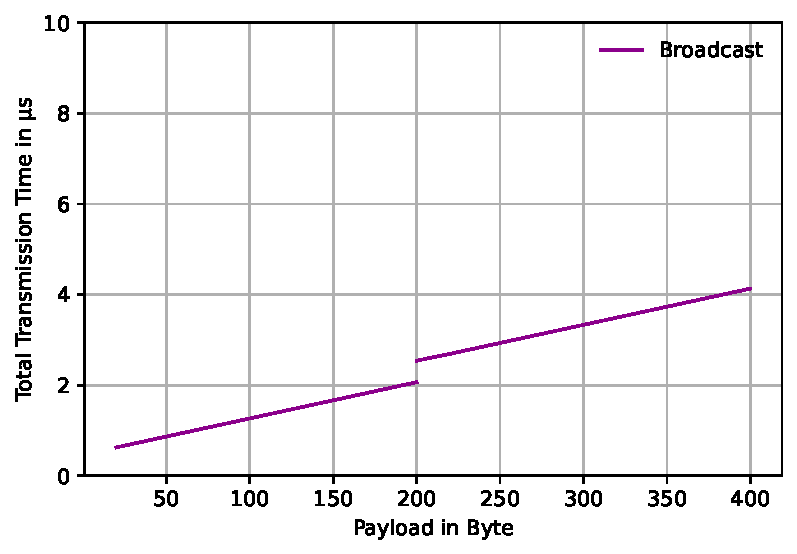
\includegraphics[scale=0.6]{/home/walther/Documents/bachelor/Plot2/Graphs/bc_analytic.pdf}
	\caption{Transmission Time of Broadcasts Depending on Payload}
	\label{fig:bc_analytic}
\end{figure}

Due to the fact that a second broadcast is needed if the maximum payload of ESP-NOW is exceeded,
the expected transmission time is not continuous, as shown in \cref{fig:bc_analytic}.
It is easy to see that the additional overhead caused by adding another package creates noticeable latency.

\subsubsection*{Update Frequency}

However, while compareing this to the latency of unicast \ref{tab:airtime_unicast_calc},
it becomes clear that the low overhead and the missing acknoledgements lead to a significantly higher rate.
A complete pass, i.e. addressing all WESs with 20 bytes, is already an order of magnitude faster from a number of 10 WESs.

\begin{align}
	\text{Frequency}_{UC} &= \frac{1}{10 \cdot 1270\mu s} = 78.7 Hz \\
	\text{Frequency}_{BC} &= \frac{1}{2456\mu s} = 407.2 Hz
\end{align}

Even if these values are only remotely comparable with real measurement data, it is clear,
that the throughput is significantly higher with broadcast than with unicast.
This effect should be even clearer under real conditions.

\begin{figure}[h]
	\centering
	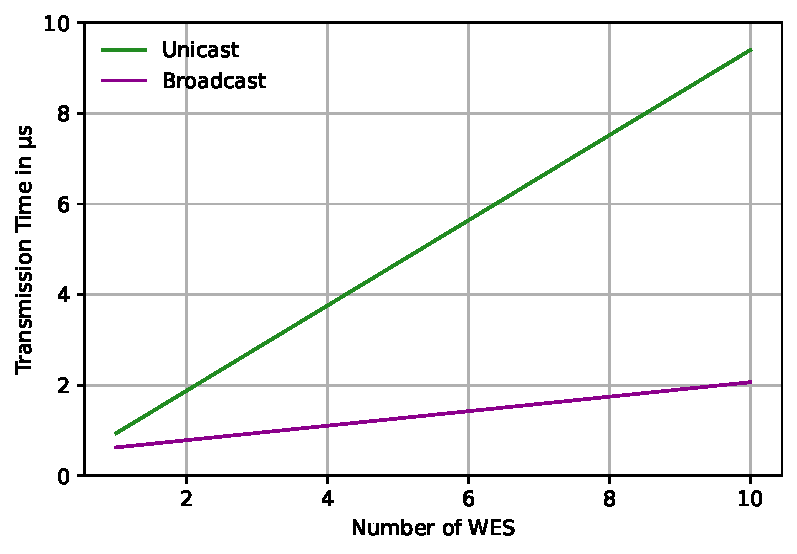
\includegraphics[scale=0.6]{/home/walther/Documents/bachelor/Plot2/Graphs/bc_uc_transmissiontime_analytic.pdf}
	\caption{Transmission Time of Unicast vs Broadcast}
	\label{fig:bc_uc_transmissiontime_analytic}
\end{figure}

\subsubsection*{Reliability}

The huge advantage that the Slim Broadcast has over the Slim Unicast in terms of update frequency,
comes at the cost of lower reliability.
Broadcasts can't do acknolegements,\todo{ref to fundamentionals, datalink, broadcast}
a WES that has poor reception to the controller, will not receive packets and the controller cannot take countermeasures.
\cref{sec:DLbroadcast}

\subsubsection*{Synchronisation}
Insead of transmitting to several fixtures after each other slim broadcast just transmitts to all fixtures at the same time.
This solves the problem of synchronization for less than 200 channel.
For more than 200 each WES has to wait until the last broadcast has arrived.
In contrast to unicast, the buffering delay can be calculated almost deterministically for broadcast 
due to the absence of automatic retransmissions.

\subsection*{Rapid Repetition}

\todo{Is Rapid Repetition a appropriate name? Unsosliced Repetition is better siehe Paper?}

To improve the reliability of the slim broadcast, the same transmission can simply be repeated unsolicited.
The idea is not to wait for a missing acknolegedment, but to increase the probability that one of the packets got through.
\todo{Cite paper A First Implementation and Evaluation of the IEEE 802.11aa Group Addressed Transmission Service}
The reliability of the Slim Broadcast with Rapid Repetition is improved with every rapid repetition (RR).
In the formula below \cref{math:rr_sr}, with RR set to zero, there happens no repetition.

\begin{figure}[h]
	\centering
	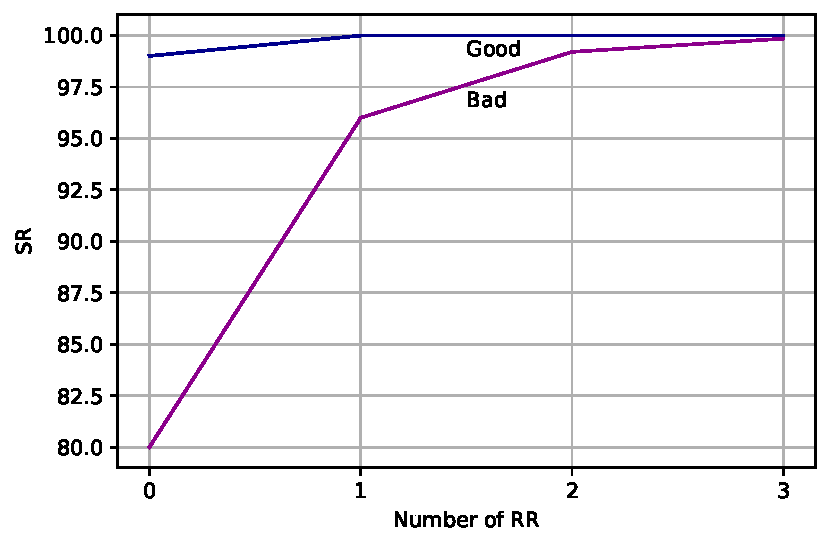
\includegraphics[scale=0.6]{/home/walther/Documents/bachelor/Plot2/Graphs/theory_sr_rr.pdf}
	\caption{Success Ratio increase with increasing number of RR}
	\label{fig:theory_rr_sc}
\end{figure}

\begin{align}
	\label{math:rr_sr}
	\text{SR}_{RR}(RR)	&= 1-(1-\text{SR})^{RR+1} \\
	\text{SR}_{RR}(0) 	&= SR \\
	\text{SR}_{RR}(1) 	&= 1-(1-\text{SR})^{2}
\end{align}

The RR makes it possible to reach WESs with poor reception much more reliably,
However, WESs that have very good reception also receive the same packet redundantly.
The update frequency of a BC with RR must be divided by the number of repetitions, compared to one without repetitions,
the same applies to the latency when synchronisation is required.
However, in contrast to unicast, broadcast offers such shorter transmission times,
that at least a few repetitions can be accepted. \cref{fig:rr_analytic}

\begin{figure}[h]
	\centering
	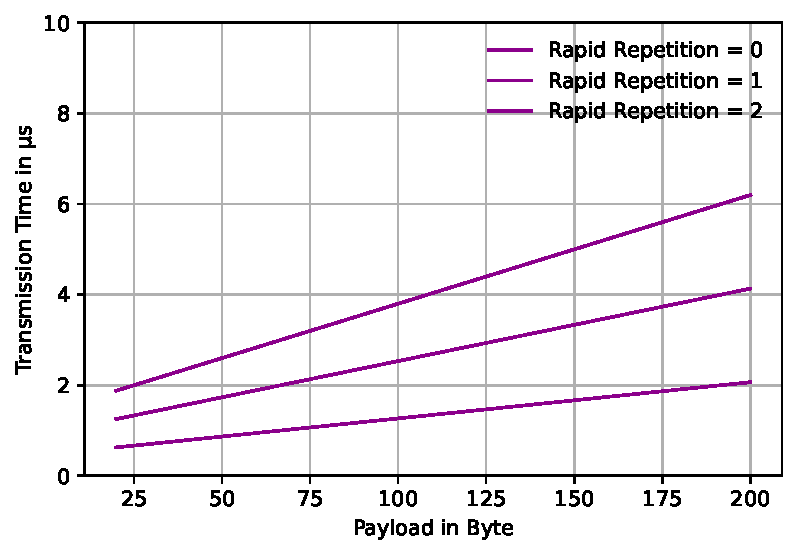
\includegraphics[scale=0.6]{/home/walther/Documents/bachelor/Plot2/Graphs/rr_transmission_time.pdf}
	\caption{Transmission Time with with different sets of RR over rising Payload}
	\label{fig:rr_analytic}
\end{figure}

\subsection*{Delayed Rapid Repetition}
\label{sub:DelayedRepetition}

To push the idea of rapid repetion even further, should also temporarily occuring noise be taken into account.\todo{displaced repetition vs delayed repetition}
This can cause all the repetitions to be captured at once.
If the individual repetitions of the first sequence are sent displaced together with those of the second sequence,
then the probability that at least one of the repetitions is not detected by a occuring noise noise is increased.

By staggering the individual sequences, the update frequency is not affected,
because just as many packets are sent as with Slim Broadcast RR.
The latency, on the other hand, is significantly increased, especially when synchronisation is maintained.
In the given example of \cref{fig:badChannel} the WESs has to wait for 5 times the duration of a broadcast transmission, instead of three.

\begin{figure}[h]
	\centering
	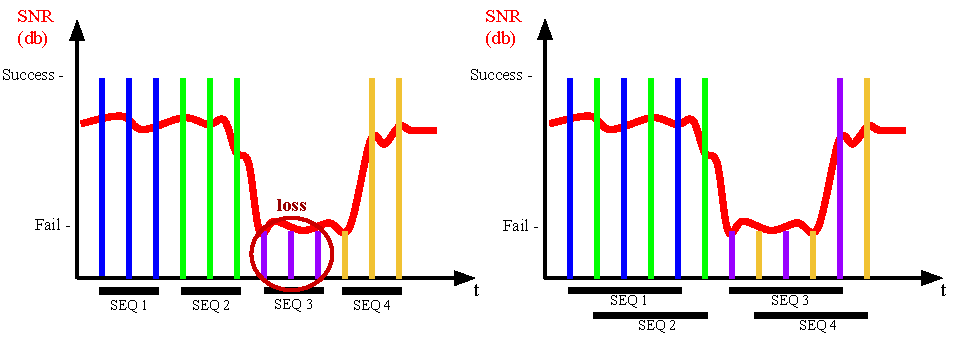
\includegraphics[scale=0.75]{figures/BadChannel.pdf}
	\caption{Rapid Repetition = 3 over a occuring noise}
	\label{fig:badChannel}
\end{figure}

The delay of the Delayed Rapid Repetition (DR) can also be extended considerably.
In extreme cases, it could be set to the number of sequences, which is of course impractical,
but interleaving two or three sequences could help counteract persistent noise.

\begin{figure}[h]
	\centering
	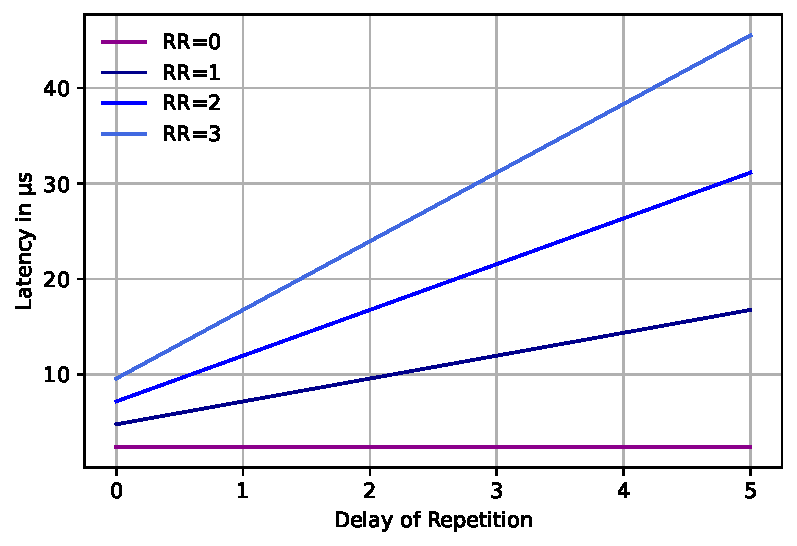
\includegraphics[scale=0.60]{../Plot2/Graphs/bc_dr.pdf}
	\caption{Latency of DR, transmitting 200 Byte}
	\label{fig:dr_delay}
\end{figure}

With DR, improved reliability comes at the cost of latency, not update frequency,
because no more packets are sent, only the order is shifted.
If no repetition is applied, the delayed rapid repetition has no influence,
which is why the graph \cref{fig:dr_delay} remains constant for RR=0.
The greater the RR and the delay of the DR, the more packets where send
between the first and the last packet of each sequence.

The measurement results \cref{sec:evaluation} will show whether the use of delayed repetition 
can reduce the number of rapid repetitions while maintaining or even improving reliability.

\section{Implementation}

The developer boad ESP32 Devkit V1 used in the experiments (\cref{sec:evaluation}) for the collection of the data
can be ordered cheaply 
\footnote{3.79€, www.aliexpress.com, ESP32 Devboard V1, 3/3/22}
from common (most favourably Chinese) websites. 
The most accessible way to flash a chip is using the Arduino IDE, which can be easy configured for flashing ESPs.
A more precise approach is to use the IDF of Espressif itself, 
which can also be easily made to work by installing the toolchain and build tools and an Plugin for your favorite IDE.

\begin{figure}[h]
	\centering
	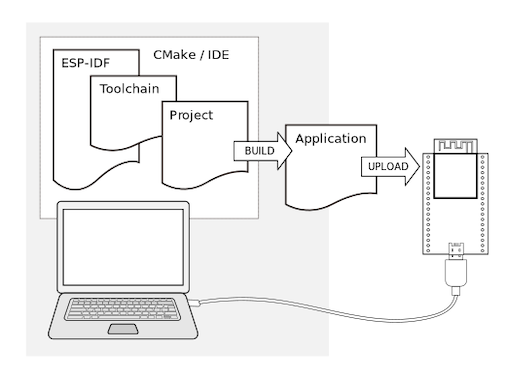
\includegraphics[scale=0.4]{figures/ESP-ISF.png}
	\caption{Flashing ESP}
	\label{fig:ESP-IDF}
	\footnote{\url{https://docs.espressif.com/projects/esp-idf/en/latest/esp32/_images/what-you-need.png, 3.3.2022}}
\end{figure}

Espressif has provided a user guide for the use of ESP-NOW ~\cite{ESPNOWGuide},
but unfortunately it contains some of informations which are outdated, 
for example, it claims that broadcast is not supported.
However, more detailed information can be found on the website.
% \footnote{\url{https://docs.espressif.com/projects/esp-idf/en/latest/esp32/api-reference/network/esp_now.html}}.

To use ESP-NOW on an ESP, only a few steps are necessary.
The chip must activate Wifi and put it in STA mode and ESP-NOW can be activated.
The two libraries "esp\_wifi.h" and "esp\_now.h" are required for this.

\begin{lstlisting}[caption=Init ESP-NOW]
WiFi.mode(WIFI_STA);
esp_now_init();
\end{lstlisting}
\label{lst:init}

\todo{check formatation in the final version}

Later, the individual MAC addresses of the WESs must be saved.
These are created in a separate header file and can then be added during the setup of the chip.
The MAC address is needed to add the respective WES to the peerlist.
However, the WES does not have to be switched on or within range for this, it is more a case of making the WES known to the controller.
The Controller can store up to 20 devices in his peerlist at the same time.

\todo{listing box prevent linebreaks on newpage}
\begin{lstlisting}
#ifndef MACLIST_H
#define MACLIST_H

uint8_t WES_MAC_1[6] = { 0xFC ,0xF5 ,0xC4 ,0x31 ,0x9A ,0x44 };
uint8_t WES_MAC_2[6] = { 0x24, 0x0A, 0xC4, 0x61, 0x19, 0x08 };
uint8_t BC_MAC[6]    = { 0xFF, 0xFF, 0xFF, 0xFF, 0xFF, 0xFF };
\end{lstlisting}
\label{lst:macaddress}

\begin{lstlisting}[caption=Add Peers]
#include "maclist.h"

if (!esp_now_is_peer_exist(WES_MAC_1)) {
  peer_info.channel = 13;                   // 1-14
  memcpy(peer_info.peer_addr, WES_MAC_1, 6);
  esp_err_t status = esp_now_add_peer(&peer_info);
}
if (ESP_OK == status) {                     // check success
  Serial.println("[OK] Slave-peer added"); 
}
\end{lstlisting}

Sending an ESP-NOW unicast is performed with the method esp\_now\_send().
The MAC address of the recipient is passed, a pointer to the payload to be transmitted and its length.
In the case of a broadcast, the address field is filled with the broadcast address ff:ff:ff:ff:ff:ff),
The function esp\_now\_register\_send\_cb can be used to check whether the cast was successfully sent out.
It is important to write as little code as possible in such a callback function.
If you send the next package only after receiving the dispatch confirmation, then you can be sure that the packages are sent in the correct format,
that the packages are sent in the correct order.

\begin{lstlisting}[caption=Send ESP-NOW Cast UC/BC]
void metaInformationToSlaves(const uint8_t *peer_addr, struct_advanced_meta metaData) {
  esp_now_register_send_cb(onDataSent);     // register callback

  esp_err_t status = esp_now_send(WES_MAC_1,
                                 (uint8_t *) &payload,
                                 sizeof(payload));
  if (ESP_OK == status) {                   // check success
    Serial.println("[OK] ESP-NOW sending"); 
  }

void onDataSent(const uint8_t *mac_addr, esp_now_send_status_t status) {
  if (status == ESP_NOW_SEND_SUCCESS) {
    Serial.println("[OK] ESP-NOW Send"); 
  }
}
\end{lstlisting}
\label{lst:sendcast}

Working with mirocontrollers requires a non continous program-flow, instead it's event-based.
For the individual WESs, a callback function is registered after setup, 
it's called when an ESP-NOW transmission is passed on to the application layer.

\begin{lstlisting}[caption=ESP-NOW Callback Functions]
esp_now_register_recv_cb(OnDataRecv);

void OnDataRecv(const uint8_t *mac_addr, const uint8_t *incomingData, int data_len) {
  if (incomingData[0] == 253) {             // setup data
    applyMetaInformation(incomingData, data_len);
    return;
  }
  if (incomingData[0] == 255) {             // verify data
    applyPayload(incomingData, data_len);
  }
  if (incomingData[0] == 254) {             // return results
    sendResultsToMaster();
    return;
  }
\end{lstlisting}
\label{lst:callback}
